\documentclass{article}
\usepackage[english]{babel}
\usepackage[utf8]{inputenc} %utf-8
\usepackage[a4paper, total={5.5in, 9in}]{geometry}
\usepackage{url}
\usepackage{graphicx}
\usepackage[table]{xcolor} %Color en las celdas
\usepackage{subcaption}
\usepackage{appendix}
\usepackage{booktabs}
\usepackage{enumitem}
\usepackage{rotating}
\usepackage{listings}
\usepackage{xcolor}

\colorlet{punct}{red!60!black}
\definecolor{background}{HTML}{EEEEEE}
\definecolor{delim}{RGB}{20,105,176}
\colorlet{numb}{magenta!60!black}

\lstdefinelanguage{json}{
	basicstyle=\normalfont\ttfamily,
	numbers=left,
	numberstyle=\scriptsize,
	stepnumber=1,
	numbersep=8pt,
	showstringspaces=false,
	breaklines=true,
	frame=lines,
	backgroundcolor=\color{background},
	literate=
	*{0}{{{\color{numb}0}}}{1}
	{1}{{{\color{numb}1}}}{1}
	{2}{{{\color{numb}2}}}{1}
	{3}{{{\color{numb}3}}}{1}
	{4}{{{\color{numb}4}}}{1}
	{5}{{{\color{numb}5}}}{1}
	{6}{{{\color{numb}6}}}{1}
	{7}{{{\color{numb}7}}}{1}
	{8}{{{\color{numb}8}}}{1}
	{9}{{{\color{numb}9}}}{1}
	{:}{{{\color{punct}{:}}}}{1}
	{,}{{{\color{punct}{,}}}}{1}
	{\{}{{{\color{delim}{\{}}}}{1}
	{\}}{{{\color{delim}{\}}}}}{1}
	{[}{{{\color{delim}{[}}}}{1}
	{]}{{{\color{delim}{]}}}}{1},
}



\graphicspath{{img/}}

\bibliographystyle{unsrt}

% Header and footer
\usepackage{fancyhdr}
\fancyhf{} % sets both header and footer to nothing
\renewcommand{\headrulewidth}{0pt}
\fancyhead[LE,RO]{Share\LaTeX}
\fancyhead[RE,LO]{Guides and tutorials}
\fancyfoot[CE,CO]{\leftmark}
\fancyfoot[LE,RO]{\thepage}

% todo command
\newcommand{\todo}[1]{\textbf{\textit{\color{red}#1}}}



\begin{document}
\begin{center}
	\begin{Huge}
	\textbf{Software Development}\\
	\end{Huge}
	\begin{small}
		\textbf{Submission 3: Prototyping, Review and Planning}
	\end{small}
\end{center}

\begin{small}
\textit{\\Exam Nº: B126551}\\
\today
\end{small}

\begin{center}
	\noindent\rule[0.5ex]{\linewidth}{1pt}
\end{center}

\section{Prototype}
The prototype we have developed demonstrates the capabilities of the game to be developed. Originally it was intended to be a Unity game (standalone or web application), but due to difficulty of implementation we have decided to implement it on Python 2. While Unity is a solution for both functionality and user interface, we have used pure Python 2 code for functionality and will use \texttt{PyJs} to develop the user interface. PyJs is a Rich Internet Application Development Platform for both Web and Desktop. It is able to compile Python code to Javascript so we can create a web application in Python. It comes in web and desktop versions in case we want to run in on a browser or as a standalone application. All the code developed for this assignment can be found at \url{https://github.com/iAbadia/SD-ASSESSMENT-3}.

The prototype implements all the necessary classes to represent the elements inside the game:
\begin{itemize}
	\item \textbf{User.} The \texttt{User} object represents a real user. It has a username, a password and an about (or description) section.
	\item \textbf{Squad.} A \texttt{Squad} is formed by many attributes such as the name, whether it is private or public, the available credits, etc. It also has a \texttt{Captain} and a \texttt{Hierophant}, a list of \texttt{Teammembers} and a stash, which is a list of \texttt{Item}.
	\item \textbf{Captain and Hierophant.} These classes are very similar. They have a name, experience, a list of skills, stats (Health, Fight, Move, etc.) and a list of \texttt{Item}.
	\item \textbf{Teammember.} This class represents the playable characters that are nor a Captain or a Hierophant. They have a name and stats.
	\item \textbf{Item.} This represents the items inside the game. It has a name, a cost, a type and value. The meaning of the value depends on the type, if it is a weapon it is damage, but if it is a health potion it is how much health it restores.
	\item \textbf{Fight.} This class represents a battle. It has two squads and helps keep track of the battle actions, inflict damage on players, change turn or save the squads once finished.
	\item \textbf{Configuration.} This class stores the application configuration such as low resolution mode or colorblind mode.
\end{itemize}

We have also implemented a set of functions as an interface between these Python Objects and the persistence layer which has been implemented as JSON files (see appendix \ref{app:json} for an example of how a squad is stored). These functions will both read a JSON file and return it, find a specific value in the file and return it or save a JSON variable to a file. These files are gathered under the folder \texttt{resources}:

\begin{itemize}
	\item \texttt{\textbf{config.json:}} Stores the values for low resolution, reduced flickering and colorblind modes.
	\item \texttt{\textbf{cpt-spec.json, hpt-spec.json:}} These files contain the lists of available Captains and Hierophants along with their names, stats, cost, skill trees and the skills available within them.
	\item \texttt{\textbf{items.json:}} This file stores the available items in the game.
	\item \texttt{\textbf{squad-members.json:}} Just like \texttt{cpt-spec/htp-spec} this file contains the available team members along their cost, name, stats, etc.
	\item \texttt{\textbf{users.json:}} Stores the list of created local users.
	\item \texttt{\textbf{squads:}} This folder contains one JSON file per user and stores their squads. Each squad contains the Captain, Hierophant, team members, stash, credits, etc. The Captain, Hierophant, team members and items each have a Unique Identifier that helps differentiate them. Using an Object Oriented Programming analogy, we could think of the data stored in \texttt{cpt-spec}, \texttt{hpt-spec}, \texttt{squad-members} and \texttt{items} as classes and the data in files in the \texttt{squads} folder as instances of those classes.
\end{itemize}

Using JSON files helps keep an easily updatable list of Captains, Hierophants and team members.

\subsection*{Prototype demonstration}
Since we have not implemented a user interface yet, the prototype demonstration is performed via a scripted series of ``user events''. We have implemented five use cases within the \texttt{main.py} file. The demonstration can be run by executing \texttt{python main.py} within the project's \texttt{src} folder. We have also included backup user files in case the demonstration is run too many times that the squads run out of credits.

\paragraph{User login.} This use case takes two users an tries to log them in. The first one inputs the right user and password so we get a valid user, the second inputs the password wrong the first time so it gets an invalid User object. There is a second attempt where the second user logs in successfully. The output of this use case can be observed on Listing \ref{lst:user-login}.

\begin{lstlisting}[caption={User login use case output.},label={lst:user-login},captionpos=b,frame=single]
User1 authenticated!
User2 failed login!
User2 authenticated!
\end{lstlisting}

\paragraph{Edit user.} This use case prints the about section of a user, edits it and saves it. It then recreates the \texttt{User} object and prints the modified about section. The change can be observed in an included random integer at the end (see lst. \ref{lst:user-edit}).

\begin{lstlisting}[caption={User edit use case output.},label={lst:user-edit},captionpos=b,frame=single]
User1 authenticated!
Old user1 about: This is the new user1 about [378]
User1 authenticated!
New user1 about: This is the new user1 about [298]
\end{lstlisting}

\paragraph{Edit configuration.} This time we create a \texttt{Config} object and print the values for the configuration options. We then invert them (since they are boolean values), recreate the configuration object and print again the values (see lst. \ref{lst:config-edit}).

\begin{lstlisting}[caption={User configuration use case output.},label={lst:config-edit},captionpos=b,frame=single]
INITIAL CONFIGURATION
---------------------
Colorblind:    True
Lowres:        True
Reduceflicker: True

FINAL CONFIGURATION
---------------------
Colorblind:    False
Lowres:        False
Reduceflicker: False
\end{lstlisting}

\paragraph{Edit squad.} This use case edits a squad by adding a new team member. We first create the Squad from a user squad list, attempt to include a team member listed in the file \texttt{squad-memeber.json} that costs more than the credits the squad has available. We print the squad to check that the team member has not being added and then add an affordable team member (see lst. \ref{lst:squad-edit}).

\begin{lstlisting}[caption={Squad edit use case output.},label={lst:squad-edit},captionpos=b,frame=single]
-------------- SQUAD ----------------
Name:    Squad 1 from User 1
Owner:   user1
UID:     1f3b187ca90344d383b486a7ebdb355c
Private: False
Credits: 2001
------------ CAPTAIN ---------------
Name:    Warlord
ID:      006-00001
UID:     aed2cbfcaa9f4400b236f055787ffbe2
XP:      300
----------- HIEROPHANT -------------
Name:    Priest
ID:      007-00001
UID:     09404448f6654703ac234f1d542198d4
XP:      500
------------- ROSTER ---------------
This guy 1    | 005-00002 | Main: False
This guy 2    | 005-00003 | Main: False
------------- STASH ----------------
Power potion  | 001-00001 |  10 (cost) | 20 (value)
Bow of Mordor | 002-00002 | 230 (cost) | 25 (value)

Member 005-00004 not added!

-------------- SQUAD ----------------
Name:    Squad 1 from User 1
Owner:   user1
UID:     1f3b187ca90344d383b486a7ebdb355c
Private: False
Credits: 2001
------------ CAPTAIN ---------------
Name:    Warlord
ID:      006-00001
UID:     aed2cbfcaa9f4400b236f055787ffbe2
XP:      300
----------- HIEROPHANT -------------
Name:    Priest
ID:      007-00001
UID:     09404448f6654703ac234f1d542198d4
XP:      500
------------- ROSTER ---------------
This guy 1    | 005-00002 | Main: False
This guy 2    | 005-00003 | Main: False
------------- STASH ----------------
Power potion  | 001-00001 |  10 (cost) | 20 (value)
Bow of Mordor | 002-00002 | 230 (cost) | 25 (value)

Member 005-00003 added!

-------------- SQUAD ----------------
Name:    Squad 1 from User 1
Owner:   user1
UID:     1f3b187ca90344d383b486a7ebdb355c
Private: False
Credits: 2001
------------ CAPTAIN ---------------
Name:    Warlord
ID:      006-00001
UID:     aed2cbfcaa9f4400b236f055787ffbe2
XP:      300
----------- HIEROPHANT -------------
Name:    Priest
ID:      007-00001
UID:     09404448f6654703ac234f1d542198d4
XP:      500
------------- ROSTER ---------------
This guy 1    | 005-00002 | Main: False
This guy 2    | 005-00003 | Main: False
Demoman       | 005-00003 | Main: False
------------- STASH ----------------
Power potion  | 001-00001 |  10 (cost) | 20 (value)
Bow of Mordor | 002-00002 | 230 (cost) | 25 (value)
\end{lstlisting}

\paragraph{Simulate battle.} This use case creates a \texttt{Fight} object and simulates a Captain from team A attacking a Hierophant from team B. We then end the game and save the squad, recreate the \texttt{Fight} object and check that the Hierophant's health have been decreased by the same amount that the Captain inflicted damage (see lst. \ref{lst:sim-fight}).

\begin{lstlisting}[caption={Simulate battle use case output.},label={lst:sim-fight},captionpos=b,frame=single]
User1 authenticated!
User2 authenticated!
User1 will use Squad <7911ceb9f0f546c2b49bff6a8bd7044d>
User2 will use Squad <b3f175ec05564cdbbb8545bf6f26b469>
Squad B Hierophant health pre-fight:  400
Squad A Captain attacks with 50 damage
Squad B Hierophant health post-fight: 350
\end{lstlisting}

\section{Review}
The prototype showed in this document has deviated from the original plan. As we already explained at the beginning of the document, we have decided to use \texttt{Python} + \texttt{PyJs} instead of Unity. This decision has helped us avoid the learning curve that Unity involves for new developers. 

Another important aspect of the development is networking, which we have not implemented yet. The prototype is only capable of local battles, although the design we have followed is easily adaptable to include a battle over the network. We estimated that this feature is not crucial when it comes to show the potential of the game.

The class diagram that we designed on the first assignment has been followed without issues since, even we changed the implementation language, we are still using the Object Oriented Programming paradigm. In the other hand, the persistence layer was planned to be implemented with a \texttt{SQLite} database but we have finally decided to use plain text JSON files. Adapting to a more complex persistence layer (like going back to the original plan and use SQLite) may be required in the future, this is why we have meticulously implemented a persistence interface in the file \texttt{persistence.py} so only this file would require modification.

Regarding the original time planning, we have had to drastically alter the expected progress. The first design was intended to use Unity as the game engine which involves a big learning curve that, once overcome, helps build the game quicker than using just Python. This made us replace the Unity learning period with game resources design (files \texttt{cpt-spec}, \texttt{hpt-spec}, \texttt{items}, etc.) and functionality implementation.

\section{Planning}
This section includes the time planning for the project as well as the risk analysis.

\subsection*{Time planning}
Figure~\ref{fig:gantt} shows the Gantt chart for the project. We have broke down the task list into five categories: Setup, Implementation, Art, Documentation and Public testing. The prototype shown in this document would be results of this planning until \texttt{Persistence} task within the \texttt{Implementation} category. We have adapted the previous schedule to our plan (use Python and PyJs instead of Unity).

\begin{figure}
	\centering
	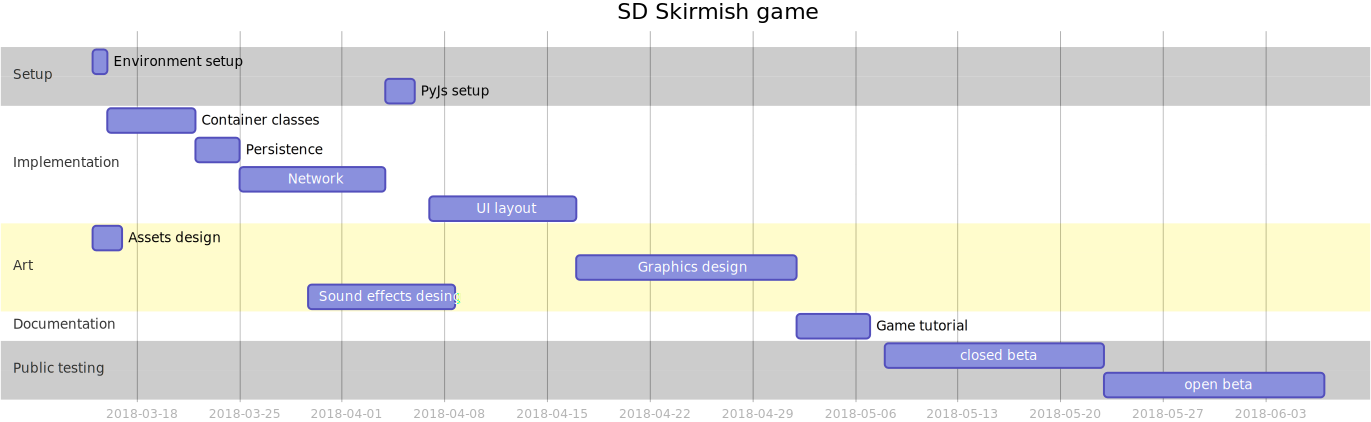
\includegraphics[width=.99\textwidth]{gantt}
	\caption{Gantt chart for the project.}
	\label{fig:gantt}
\end{figure}

\subsection*{Risk analysis}
The new changes we have performed on the project plan have also yielded new problems. Table \ref{tab:risks} shows the list of risks we have identified for the development and testing periods, prior to the game launch.

\begin{table}
	\centering
	\begin{tabular}{p{4cm}|p{1.5cm}p{5.5cm}p{1.5cm}p{1cm}}
		\toprule
		Risk                                            & Control & Contingency                                                                                                               & Likelihood & Impact   \\ \midrule
		JSON Resources become too complicated to handle & Control & Migrate to a SQL database and reimplement the persistence interface.                                                      & Medium     & High     \\
		PyJs goes out of development                    & Control & We will have to migrate our UI to another solution                                                                        & Very Low   & Critical \\
		Art designed leaves the team                    & Avoid   & We will keep our art designer happy and willing to continue working on this project                                       & Low        & Medium   \\
		Beta testing period extended                    & Accept  & The beta period is set to last one month. We expect to fix most issues in that time period but we might require more time & Medium     & Medium
	\end{tabular}
	\caption{List of risks identified.}
	\label{tab:risks}
\end{table}


\begin{appendices}
\section{Squad JSON}
\label{app:json}
\begin{lstlisting}[language=json]
{
  "hierophant":{
    "stats":{
      "shoot":30,
      "armour":300,
      "move":10,
      "fight":50,
      "morale":60,
      "health":600
    },
    "uid":"09404448f6654703ac234f1d542198d4",
    "skills":[
    "007-01001"
    ],
    "items":[
    {
      "uid":"b4dea62aded64e0fa3597cd0b2dc5d7a",
      "value":200,
      "name":"Baton of Destiny",
      "cost":3000,
      "type":[
      "baton",
      "legendary"
      ],
      "id":"004-00001",
      "description":"This baton belonged to the ultimate Destiny Priest."
    }
    ],
    "xp":500,
    "id":"007-00001",
    "name":"Priest"
  },
  "uid":"1f3b187ca90344d383b486a7ebdb355c",
  "roster":[
  {
    "uid":"fc9feeb2a9814e16bc37fb7558f336f8",
    "main":false,
    "stats":{
      "shoot":30,
      "armour":15,
      "move":10,
      "fight":50,
      "morale":60,
      "health":60
    },
    "id":"005-00002",
    "name":"This guy 1"
  },
  {
    "uid":"26e3d1d7bcde486d94a403c9e6769bc2",
    "main":false,
    "stats":{
      "shoot":30,
      "armour":300,
      "move":10,
      "fight":50,
      "morale":60,
      "health":600
    },
    "id":"005-00003",
    "name":"This guy 2"
  }
  ],
  "stash":[
  {
    "uid":"34a871cb3dc84d7b9a47ab8b3a0e1639",
    "value":20,
    "name":"Power potion",
    "cost":10,
    "type":[
    "heal",
    "potion"
    ],
    "id":"001-00001",
    "description":"Restore 20 HP."
  },
  {
    "uid":"4d1d5df6159a47289765e323d11957cc",
    "value":25,
    "name":"Bow of Mordor",
    "cost":230,
    "type":[
    "bow",
    "longbow",
    "elf-weapon"
    ],
    "id":"002-00002",
    "description":"The legend says that it belonged to the mighty Legolas."
  }
  ],
  "credits":1901,
  "private":false,
  "owner":"user1",
  "captain":{
    "stats":{
      "shoot":30,
      "armour":300,
      "move":10,
      "fight":50,
      "morale":60,
      "health":600
    },
    "uid":"aed2cbfcaa9f4400b236f055787ffbe2",
    "skills":[
    "006-01001"
    ],
    "items":[
    {
      "uid":"c396d77a888445eaa51bcb445dce432c",
      "value":200,
      "name":"Sword of Destiny",
      "cost":3000,
      "type":[
      "sword",
      "legendary"
      ],
      "id":"002-00001",
      "description":"This sword belonged to the ultimate Destiny Samurai."
    }
    ],
    "xp":300,
    "id":"006-00001",
    "name":"Warlord"
  },
  "name":"Squad 1 from User 1"
}
\end{lstlisting}

\end{appendices}


\end{document}